\section{Construction}
The dc-motor needs a housing of some kind and a way of mounting the rotating pcb.
These mounts were chosen to be 3D printed, due to the ease of doing 3D printing, if you have a 3D CAD model.

A housing was drawn in 3D, with the motor in the center, and a hole for a shaft at the side. 
A picture of the housing can be seen in figure \ref{fig:housing3D}.
The motor is then mounted with screws through the small holes in the top.

The rotating pcb is not mounted directly on the shaft of the motor due to the speed of the motor.
The motor is rated at 6000 RPM, which is too fast for the system.
Adjusting the duty cycle of the PWM which drives the motor is necessary.
Gearing the motor increases the range of duty cycles which give a desired speed.
The gear on the motor has 15 cogs and the gear on the shaft of the led board has 36 cogs, making the board spin 2.4 times slower than the motor.
This gear was mounted on a shaft that was also 3D printed, which was inserted into a bearing, mounted in the big hole in the housing.
The shaft consist of two parts, the shaft and the top.
The shaft is a rod which is inserted through the bearing and into the gear.
The top consist of a thin rod which can be inserted into the shaft and a disc which is used to mount the PCB.
The bottom PCB is then mounted between the gears and the top PCB, with the thin rod from the top going through it.
In figure \ref{fig:shaft3D} is the shaft for the board shown.

\begin{figure}[H]
 \centering
 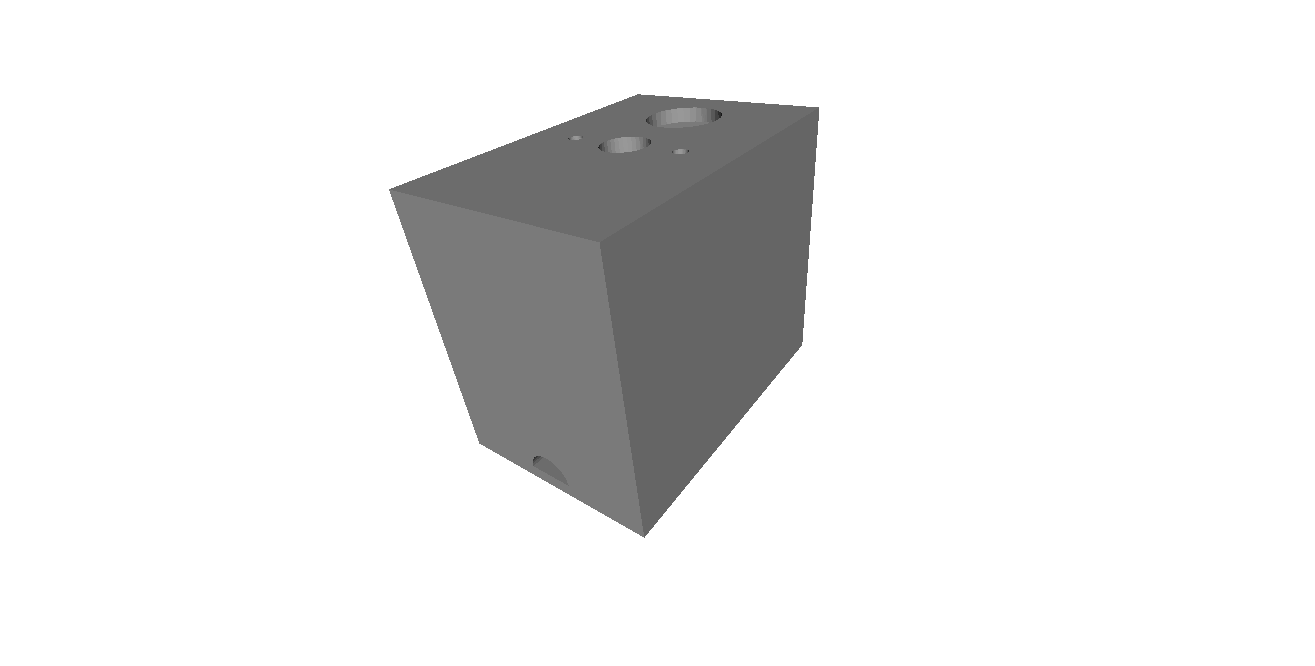
\includegraphics[width=0.7\textwidth]{img/housing3D}
 \caption{Snapshot of the housing 3D drawing.}
 \label{fig:housing3D}
\end{figure}

\begin{figure}[H]
 \centering
 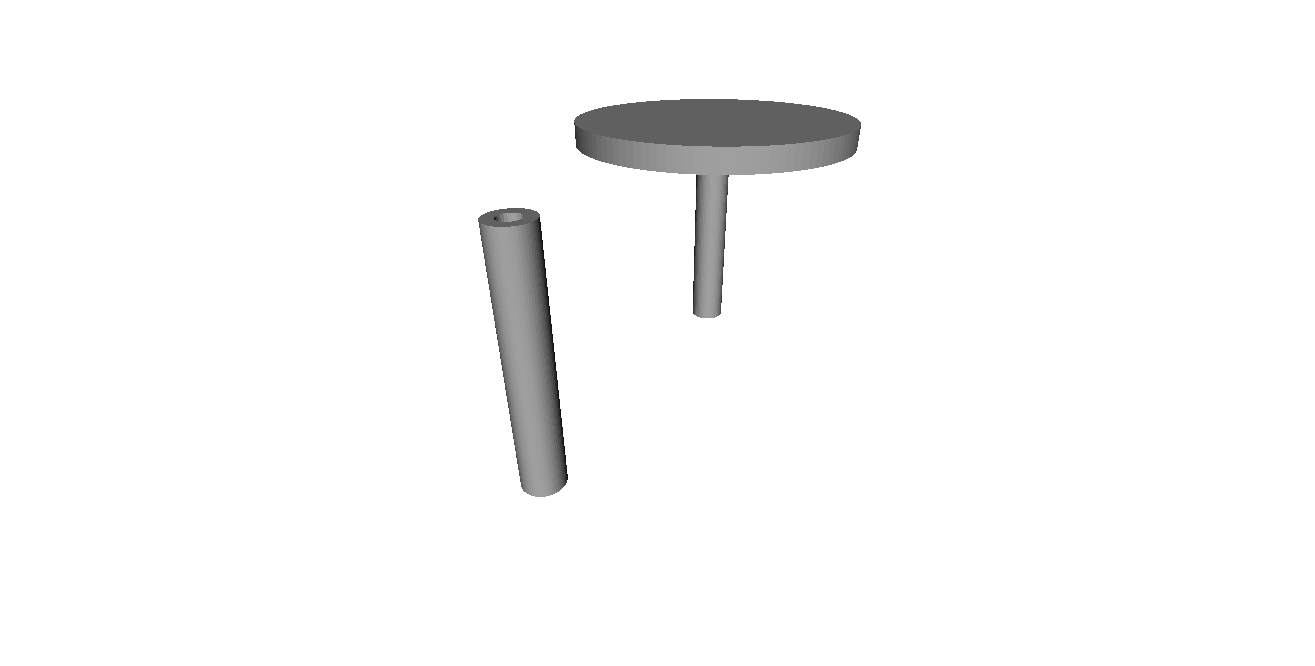
\includegraphics[width=0.7\textwidth]{img/shaft_3d}
 \caption{Snapshot of the shaft 3D drawing.}
 \label{fig:shaft3D}
\end{figure}

When running at high speed, it is important to make the system as stable as possible to reduce shaking.
One way to do this is to make the board twice the length, so the shaft goes through the center of the board, 
which should make the weight distribution almost even.
The weight of the SMD components is asummed to be negligible in relation to the weight of the PCB.